\documentclass[11pt]{article}
\usepackage[utf8]{inputenc}
\usepackage{centernot}
\usepackage[parfill]{parskip}
\usepackage{amsmath}
\usepackage{amssymb}
\usepackage{graphicx}
\begin{document}
\title{Algebra Problem 6}
\author{Robin Boregrim}
\maketitle
\renewcommand{\contentsname}{Innehållsförteckning}
\tableofcontents
\newpage
\section{Uppgiften}
Visa att linjen $(x,y,z) = (1+2t,-2t,4+3t)$ skär planet $x + 2y -2z = 7$ och bestäm skärningspunktens koordinater. Bestäm även $\sin\alpha$, där $\alpha$ är (den spetsiga) vinkeln mellan linjen och planet.
\section{Lösning}
\subsection{Beräkning av skärningspunkt}
För att hitta skärningspunkten (om det finns någon) kan börja med att stoppa in linjens uttryck för $x,y$ och $z$ i formeln för planet för att se om det finns något värde på $t$ som löser ekvationen.
  $$1+2t + 2(-2t) -2(4+3t) = 7$$
  $$1+2t - 4t -8 -6t = 7$$
  $$-8t = 14$$
  $$t = -\frac{7}{4}$$
  Om vi nu stoppar in detta värde på t i linjens formel får vi ut skärningspunkten.
  $$(x,y,z) = \Bigg(1+2\Bigg(-\frac{7}{4}\Bigg),-2\Bigg(-\frac{7}{4}\Bigg),4+3\Bigg(-\frac{7}{4}\Bigg)\Bigg)$$
  $$\Bigg(\frac{2}{2}-\frac{7}{2},\frac{7}{2},\frac{16}{4}-\frac{21}{4}\Bigg)$$
  $$\Bigg(-\frac{5}{2},\frac{7}{2},-\frac{5}{4}\Bigg)$$
  så skärningspunktens koordinater är $$(x,y,z) = \Bigg(-\frac{5}{2},\frac{7}{2},-\frac{5}{4}\Bigg).$$
\subsection{Beräkning av sin$\alpha$}
På grund av planets formel vet vi att planets normal är $$N = (1,2,-2).$$
Linjens riktings vektor $(2,-2,3)$ kan läsas av från linjens funktion.
För att beräkna vinkeln $\beta$ mellan dessa två vektorer kan vi använda oss av skalärprodukten av två vektorers egenskap att $$u \cdot v = |u||v|\cos\beta,$$
och skriva om det som $$\cos\beta = \frac{u \cdot v}{|u||v|}.$$
$$\cos\beta = \frac{(1,2,-2) \cdot (2,-2,3)}{|(1,2,-2)||(2,-2,3)|} =$$
$$\frac{2-4 -6}{\sqrt{(1^2+2^2 +(-2)^2}\sqrt{2^2 +(-2)^2 +3^2}}$$
$$-\frac{8}{\sqrt{9}\sqrt{17}}$$
$$-\frac{8}{3\sqrt{17}}$$
Så
$$\cos\beta = -\frac{8}{3\sqrt{17}}.$$
Eftersom Normalen är vinkelrät emot Planet betyder det att $$\alpha_1 = \frac{\pi}{2} - \beta.$$
$$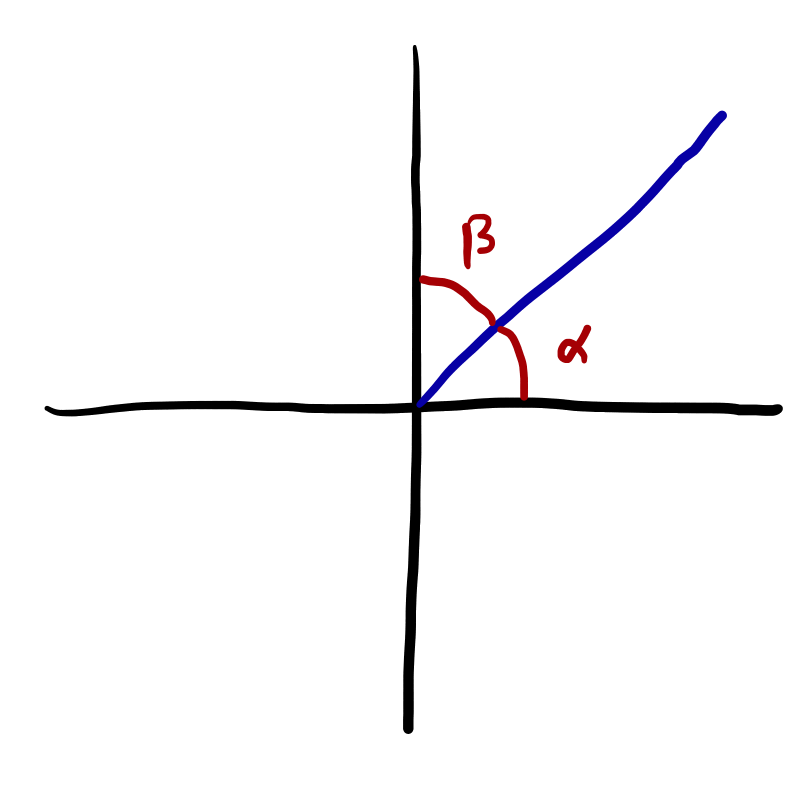
\includegraphics[scale=1]{fig1}$$
På grund av hur sinus och cosinus perioder förhåller sig till varandra så vet vi att
$$\cos(\frac{\pi}{2} - \gamma) = \sin(\gamma).$$
 Detta betyder då att $$\cos\beta =\cos(\frac{\pi}{2} - \alpha_1)= \sin\alpha.$$
 Så
 $$\sin\alpha_1 = -\frac{8}{3\sqrt{17}}$$
 Men detta sinus värde är negativt, villket betyder att vinkeln $\alpha_1$ befinner sig i antingen den tredje eller fjärde kvartalen av enhetscirkeln och är därför mycket trubbig. För att få ut $sin\alpha$ för den spetsiga vinkeln $\alpha$ så tar vi absolutbeloppet av $\sin\alpha_1$ och får:
 $$\sin\alpha = \frac{8}{3\sqrt{17}}.$$
\subsection{Svar}
Skärningspunkten för linjen och planet är: $$(x,y,z) = \Big(-\frac{5}{2},\frac{7}{2},-\frac{5}{4}\Big),$$
och sinus för den spetsiga vinkeln som linjen skär planet med är: $$\sin\alpha = \frac{8}{3\sqrt{17}}.$$
\end{document}